\subsection{Rosemary}
\paragraph{Testing the data model's flexibility}
How was the Rosemary data model changed to fit to our functional needs.
Show figure with differences.

\begin{figure}[!htb]
	\centering
	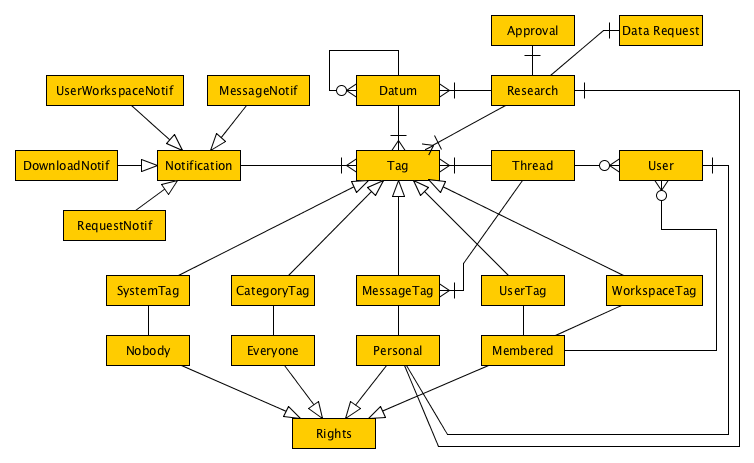
\includegraphics[width=1.0\linewidth]{images/datamodel-adapted}
	\caption{
		Rosemary data model as implemented.
		Describes workspace, tagging, datum, notification, and research models.
		The original data model can be found in figure \ref{fig:reuse-rosemary-dm}.
	}
	\label{fig:implementation-rosemary-dm}
\end{figure}

\paragraph{Back-end and front-end}
Explain how the front and back-end were changed to meet each of the functions.